\chapter{Charge Storage, Diffusion Capacitance, and Switching}
\label{ch:charge-storage-switching}

A forward-biased junction stores injected minority carriers in its neutral
regions.  Removing the forward voltage does not remove this charge
instantaneously.  Carriers must recombine or be extracted through the junction,
so current persists during switching.  The same stored-charge derivative
produces a diffusion capacitance distinct from depletion capacitance
\cite[Chap.~3, Sec.~3.5]{szeLee2012}.

\section{Stored minority charge}

For a long one-sided $p^+$--n junction, excess holes in the neutral n-region
obey $\Delta p(x)=\Delta p(0)e^{-x/L_p}$.  The stored charge per unit area is
\begin{equation}
 Q_p=q\int_0^\infty\Delta p(x)\,\dd x
 =qL_p p_{n0}(e^{V/V_T}-1).
 \label{eq:stored-minority-charge}
\end{equation}
The corresponding hole diffusion current is
\begin{equation}
 J_p=\frac{qD_pp_{n0}}{L_p}(e^{V/V_T}-1).
 \label{eq:stored-charge-current}
\end{equation}
Since $L_p^2=D_p\tau_p$,
\begin{equation}
 \boxed{Q_p=\tau_pJ_p.}
 \label{eq:charge-control-relation}
\end{equation}
This charge-control relation connects a spatial carrier distribution to a
terminal current.  For a two-sided junction, electron and hole stored charges
must both be included.

\section{Diffusion capacitance}

\begin{definition}{Diffusion capacitance}{diffusion-capacitance}
The diffusion capacitance per unit area is the small-signal derivative of
stored mobile-carrier charge:
\begin{equation}
 C_d\equiv\frac{\dd Q_s}{\dd V},
 \label{eq:diffusion-capacitance-definition}
\end{equation}
where $Q_s$ is stored minority charge per area.  It is measured in
$\mathrm{F\,m^{-2}}$.
\end{definition}

For one dominant carrier and appreciable forward bias,
\begin{equation}
 \boxed{C_d\simeq\frac{\tau_pJ_p}{V_T}.}
 \label{eq:diffusion-capacitance}
\end{equation}
Diffusion capacitance rises exponentially with forward voltage and can greatly
exceed depletion capacitance.  Under reverse bias, stored injection charge is
small and depletion capacitance dominates.

The small-signal junction model therefore contains the differential conductance
$g_d=\dd J/\dd V$, depletion capacitance $C_j$, and diffusion capacitance $C_d$.
For the ideal one-carrier diode, $C_d=\tau_pg_d$.

\begin{figure}[htbp]
 \centering
 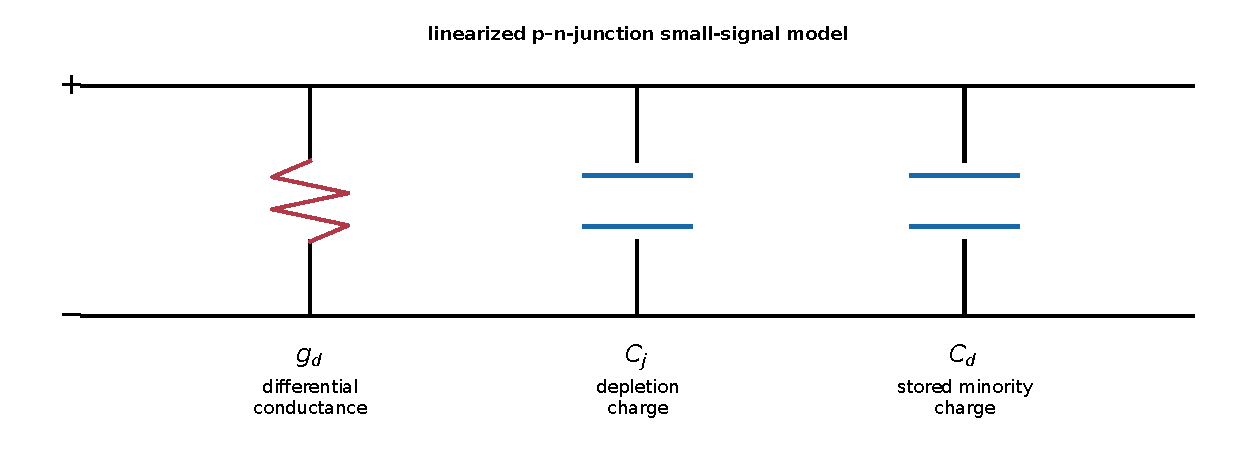
\includegraphics[width=0.88\textwidth]{figures/junction-atlas-small-signal.pdf}
 \caption{Original small-signal equivalent circuit containing differential
 conductance, depletion capacitance, and diffusion capacitance.  This is the
 physical circuit represented by Fig.~19 in Sze--Lee Chapter~3
 \cite[Sec.~3.5.2]{szeLee2012}.\figurenotebookmark}
 \label{fig:junction-atlas-small-signal}
\end{figure}
\figurenotebooktext{figures/19_charge-storage-switching/fig_19_01.ipynb}

\section{Reverse recovery}

Suppose a diode initially carries forward current and the external circuit
abruptly requests reverse current.  The junction remains effectively forward
biased while stored minority charge is being removed.  This interval is the
storage phase.  Once the depletion region is re-established, reverse current
falls during the transition phase.  The sum is the reverse-recovery time.

In a simple charge-control approximation with nearly constant reverse current
magnitude $I_R$,
\begin{equation}
 \frac{\dd Q_s}{\dd t}=I_F-I_{\mathrm{rec}}-I_{\mathrm{terminal}},
 \label{eq:charge-control-dynamics}
\end{equation}
where $I_F$ denotes injection before switching.  The actual recovery waveform
depends on the external circuit, spatial diffusion, recombination, and the
ratio of requested reverse to prior forward current.  A single lifetime is
insufficient to determine every waveform.

\begin{figure}[htbp]
 \centering
 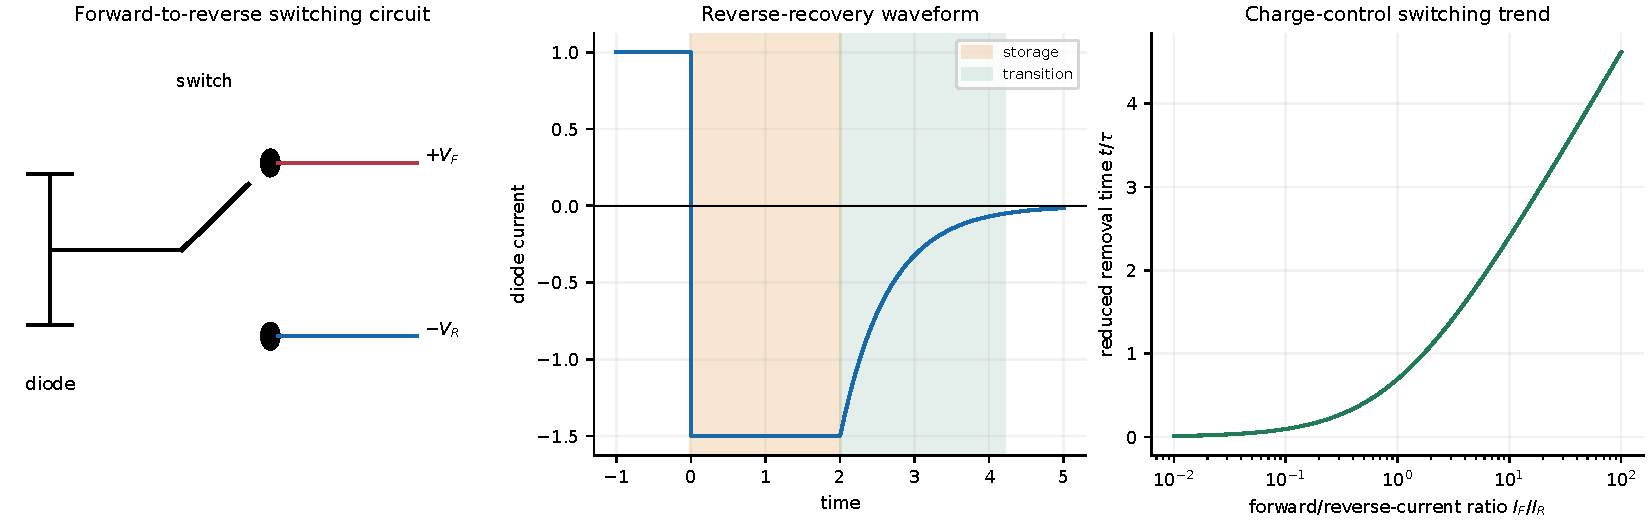
\includegraphics[width=\textwidth]{figures/junction-atlas-switching.pdf}
 \caption{Original switching circuit, reverse-recovery current waveform, and
 charge-control trend with forward-to-reverse current ratio.  The panels cover
 the physical content of Figs.~20--21 in Sze--Lee Chapter~3
 \cite[Sec.~3.5.3]{szeLee2012}.\figurenotebookmark}
 \label{fig:junction-atlas-switching}
\end{figure}
\figurenotebooktext{figures/19_charge-storage-switching/fig_19_01.ipynb}

\section{Transient finite-difference model}

After injection is removed, a neutral-region excess profile evolves according
to
\begin{equation}
 \frac{\partial\Delta p}{\partial t}
 =D_p\frac{\partial^2\Delta p}{\partial x^2}
 -\frac{\Delta p}{\tau_p}.
 \label{eq:transient-minority-diffusion}
\end{equation}
The teaching calculation initializes the finite-base steady profile from
\cref{eq:finite-base-profile}.  At $t=0$, both contacts clamp excess density to
zero.  Backward Euler advances the interior nodes:
\begin{equation}
 \left[I-\Delta t\left(D_pL_h-\tau_p^{-1}I\right)\right]
 \bm p^{k+1}=\bm p^k,
 \label{eq:transient-minority-backward-euler}
\end{equation}
where $L_h$ is the centered second-difference Laplacian.  The stored charge and
junction extraction current are
\begin{equation}
 Q_s^k=q\sum_i w_i\Delta p_i^k\Delta x,
 \qquad
 J_{\mathrm{ext}}^k\simeq qD_p\frac{\Delta p_1^k}{\Delta x}.
 \label{eq:transient-charge-current}
\end{equation}
The trapezoidal weights $w_i$ equal $1/2$ at endpoints and one inside.

\begin{figure}[htbp]
 \centering
 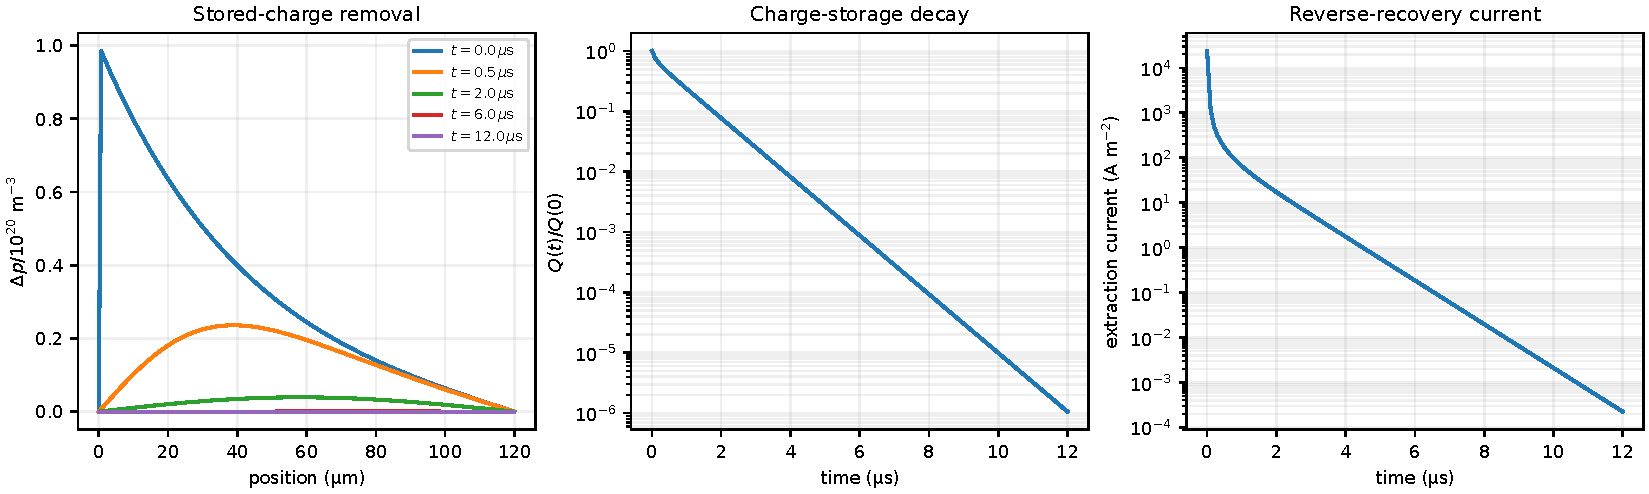
\includegraphics[width=\textwidth]{figures/junction-charge-storage.pdf}
 \caption{Removal of a stored minority-carrier profile after the injecting
 boundary is switched to equilibrium, together with total stored charge and
 extraction current.  The implicit scheme preserves nonnegative carrier
 density for the demonstrated step size.\figurenotebookmark}
 \label{fig:junction-charge-storage}
\end{figure}
\figurenotebooktext{figures/19_charge-storage-switching/fig_19_01.ipynb}

\begin{modelcheck}
With zero boundary injection and no generation, stored charge must decrease
monotonically.  Every computed density must remain nonnegative.  Integrating
\cref{eq:transient-minority-diffusion} shows that charge loss equals boundary
extraction plus bulk recombination; the notebook evaluates this balance and
performs time-step and grid-refinement checks.
\end{modelcheck}

\begin{boundarybox}
The clamped-boundary calculation isolates material diffusion and recombination;
it is not a full reverse-recovery circuit simulation.  Junction voltage,
depletion capacitance, series inductance, contact resistance, high-level
injection, and spatially varying lifetime can all alter the measured waveform.
\end{boundarybox}

\section{Chapter summary}

Forward current stores minority charge.  Its voltage derivative is diffusion
capacitance, and its delayed removal produces reverse recovery.  Charge-control
relations give compact terminal descriptions, while the transient diffusion
equation resolves spatial extraction and recombination.  Conservative charge
accounting, positivity, and refinement are the essential numerical checks.
